\chapter{Design}\label{ch:design}
This chapter will describe and explain the design of the turret, the PID controller, the detection system, the tracking system, shooting system, as well the reasoning behind them. The design is based upon the requirements in \cref{sec:requirements} and the possible solutions presented in \cref{ch:preldesign}, delimited by the hardware analysis in \cref{ch:hardware}. From this point onwards, \emph{turret} will refer to the tower described in \cref{turret}.

%The design will describe the solution which is to be implemented, but will not be directly aimed at the actual implementation of the solution.

%The design will describe the solution which is to be implemented, but will not directly address the actual implementation of the solution.

%The design will describe the solution which is to be implemented, but will not be directly aimed at the actual implementation of the solution.

%The design will describe the solution which is to be implemented, but will not target the actual implementation of the solution.

%This chapter will describe the design of the turret itself as well as its hardware and software components. The hardware components are the sensors that have to detect the moving target and inform the system about which 'zone' it is in. The software components are scheduling and the Kalman filter. The scheduling is used to control the flow of the system such that certain tasks are performed within a given time frame. The Kalman filter is responsible for converting input from the sensors into instructions for the turret which it must use to track and hit the moving target. \\ \addtodo{Mathias}{Er det for tidligt at nævne de ting? De bliver forklaret kort efter}

%All the components are designed such that they comply with the requirements listed in \cref{sec:requirements}.


\section{The Turret}\label{turret}
The turret is purpose-built using LEGO bricks following a custom design made by the project group. The turret consists of three main parts: the cannon, the tracking system and the rotation system. A total of 3 motors are mounted on the turret to aid the cannon and the rotation system. The tracking system is made up of two sensors mounted on the turret aimed in the same direction as the cannon. The turret with infrared sensors and motors mounted can be seen in \cref{turret1}. \\

\imgscale{figures/turret.png}{The turret with infrared sensors mounted}{turret1}{0.2}

The turret uses LEGO bricks as projectiles. These projectiles are fired by releasing a piston bolt from a retracted position. The bolt is pulled into a barrel by stretching elastic bands and when released it is pushed out of the barrel and into the projectile propelling it towards the target. The elastic bands are stretched using motor driven rotating rods which pass by at the apex of the stretch, releasing the bolt and allowing the elastic bands to contract. This allows for automatic fire of projectiles by continiously rotating the rods, however, it also makes priming the cannon in a cocked position somewhat difficult. The turret is loaded when the bolt is retracted as this allows a LEGO brick to drop down into the chamber just prior to the release of the bolt. The turret can hold a magazine with a capacity of 10 projectiles. The turret also allows for sensors to be mounted in various positions.

\paragraph{Projectile Accuracy} ~\\
The accuracy of the fired projectiles was tested by placing the turret 75 centimeters away from a circular target with a diameter of 5 centimeters. At this distance a projectile drop off of 10 centimeters was recorded. A total of 10 projectiles were fired and all of them managed to hit the target. The hits were not centered in one location, but spread about the target within the 5 centimeter boundary. The projectiles had some difficulty penetrating the target, a sheet of paper, at the tested distance. This can be attributed to the shape of the projectiles as well as the loss of velocity at the tested distance.

\paragraph{Motor and Sensor Selection} ~\\
Based on the motor test, see \cref{sec:actuators} and the sensor test, see \cref{sec:sensors}, the most suitable components were selected for the turret. According to the motor test the motors \textit{D} and \textit{G} are the best with the remaining motors being nearly equal in performance - with the exception of \textit{E} and \textit{C}. Motor \textit{D} has been selected as the rotation motor due to its performance, the early rotation starting point being important. Motors \textit{G} and \textit{B} have been selected for the cannon. The cannon only requires motors with similar performance from above 60\% power. \\

The turret requires sensors with a high level of accuracy. The sensors are essential in detecting the moving target and they are also used to determine the position of the target. If the two sensors interfere with each other the measurements may be incorrect resulting in the system incorrectly believing that it is tracking the target or making it unable to track the target properly. As such it is necessary to use sensors that do not interfere with each other in a manner that disrupts the readings to such an extent that the system is unable to properly track the target. As the interference between the ultrasonic sensors is too great and causes incorrect readings, these sensors have not been selected for the turret. The infrared sensors have very limited interference and they have accurate readings. Following the tests, see \cref{sec:sensors}, of both sensor types, ultrasonic and infrared, it has been determined that the infrared sensors are the most accurate \addtodo{Mathias}{Maybe - fix after sensor test} with the least amount of interference. Due to this they have been selected as the sensors of choice for the turret. 








\section{Proportional Integral Derivative Controller}\label{design:PID}
The following section will be based on \cite{PIDcontrolsystem}. In this project the proportional-integral-derivative (PID) controller will be used to make the motors more precise and able to move to a specific amount of degrees, something the motors were found to be incapable of themselves as seen in \cref{sec:actuators}. A PID controller is a commonly used control system. It can be used on a variety of systems and is popular, partly because of its robustness and simplicity, but also because it can be used in many systems with only minor changes. A PID controller is based on a control feedback loop, where the first execution of the loop only uses the current state and the goal state in the calculations. Subsequent executions of the loop uses information about the effects the previous loops had on the system.

\subsection{PID Structure}
A PID controller uses the terms \emph{P}, \emph{I} and \emph{D}, which summed up gives the change that will be applied to the actuator. \emph{P} is the proportional term, \emph{I} is the integral term and \emph{D} is the derivative term. The controller takes two inputs: the target state and the current state. The target state is the state that the PID controller is trying to reach, while the current state is the state the system is currently in. A PID controller has three coefficients: $K_p$, $K_i$, $K_d$ and two variables: \emph{lasterror} and \emph{integral}. The coefficients are part of the three terms and determine their effect on the system. An \emph{error}, see \cref{pidpseudo1}, is a number representing the difference between the current state and the target state. All errors are continuously summed up and stored in \emph{integral}. \emph{lasterror} is the error from the last state to the current state. The bigger the \emph{error} is, the more the system has to correct to reach the target state. The \emph{error} influences all the terms. \\

\emph{Proportional} is the error as it is in the current state, and it is used to make the system move towards the target. $K_p$ determines the magnitude of this term. \\

\emph{Integral} is the sum of all errors, and it increases continuously as long as the target state is not reached. Both \emph{P} and \emph{D} can reach zero if the error is sufficiently small, this problem is called steady-state error. In case of a steady-state error \emph{I} will continue to grow and will eventually start changing the system. The magnitude of the \emph{integral} term is decided by the size of $K_i$.\\

\emph{Derivative} is the difference in the error between the current state and last state, divided by the time since the last state. It is used to stabilize the system faster, as it attempts to predict the future. The magnitude of the derivative term is decided by the size of $K_d$. 


\begin{lstlisting}[style=customc, label={pidpseudo1}, caption={Pseudo code of a PID controller}]
//K_p, K_i and K_D are the PID coefficients that have been predefined
lasterror = 0
integrale = 0
PID(target, current)
    error = target - current
    integrale = integrale + error
    derivative = lasterror - error
    lasterror = error

    return Kp * error + Ki * integrale + Kd * derivative
\end{lstlisting}

\Cref{pidpseudo1} is working in the discrete time space and therefore $\Delta t$ is used in \emph{Integral} and \emph{Derivative}. In order to save calculations, $\Delta t$ has been integrated into the coefficients, this can be done as $\Delta t$ was chosen to be static.

\subsection{PID Tuning}
In order to make the PID controller work properly the three coefficients need to be tuned. There are several methods available for PID tuning, however, only two will be described here: manual tuning and the Ziegler-Nichols method. The Ziegler-Nichols method was chosen as it is a mathematically proven method~\cite{Ziegler-Nichols}, and manual tuning because it is a good way to make changes to the PID controller based on specific demands. Because these two methods are sufficient, other methods will not be explored.

\begin{table}[H]
\centering
\begin{tabular}{|l|l|l|l|}
\hline
\textbf{Control Type} & \textbf{$K_p$}     & \textbf{$K_i$}        & \textbf{$K_d$}      \\ \hline
P            & $0.50K_u$ & -            & -          \\ \hline
PI           & $0.45K_u$ & $1.2K_p/T_u$ & -          \\ \hline
PID          & $0.60K_u$ & $2K_p/T_u$   & $K_pT_u/8$ \\ \hline
\end{tabular}
\caption{Ziegler-Nichols Method}
\label{Ziegler-Nichols_Method}
\end{table}

The Ziegler-Nichols method is well defined and it is used to tune a PID controller. The first step of the method is to set $K_i$ and $K_d$ to zero. $K_p$ is then slowly increased until the motor oscillates. $T_u$ is the rate at which it oscillates, and $K_u$ is the $K_p$ value at which it oscillates. The three PID controller terms can then be calculated as shown in \cref{Ziegler-Nichols_Method}. This way of tuning is aggressive and will result in a fast rise, it might even result in some overshoot.

\begin{table}[H]
\centering
\small
\begin{tabular}{|l|l|l|l|l|l|}
\hline
           & \textbf{Rise time}    & \textbf{Overshoot} & \textbf{Settling time} & \textbf{Steady-state error}  & \textbf{Stability}              \\ \hline
$K_p$      & Decrease     & Increase  & Small change  & Decrease            & Degrade                \\ \hline
$K_i$      & Decrease     & Increase  & Increase      & Eliminate           & Degrade                \\ \hline
$K_d$      & Minor change & Decrease  & Decrease      & No effect in theory & Improve if $K_d$ small \\ \hline
\end{tabular}
\caption{Impact of increasing a parameter \cite{PIDcontrolsystem}.}
\label{Manual-tuning}
\end{table}
\FloatBarrier

Another method of system tuning is manual tuning. To use this method it is necessary to know which effect changing the coefficients has on the system. This information can be gathered from a tuning table, such as \cref{Manual-tuning}, and then the coefficients can be tuned through a trial-and-error approach or meta optimization \cite{PIDmetaOptimization}. \Cref{pidsettling} shows a graph containing the properties of a PID controller. The rise time is the time it takes for a PID controller to reach the target state for the first time, a short rise time tends to result in overshoot. Overshoot is how much a PID controller misses the target by the first time, in some systems overshoot may be prohibited. The settling time is how long it takes to reach a steady state. There might be a steady state error when there is a small error when the steady state is reached. A PID controller can be unstable and never reach a steady state which means that the coefficients have to be changed in order to stabilize the system.

\begin{figure}[H]
\centering
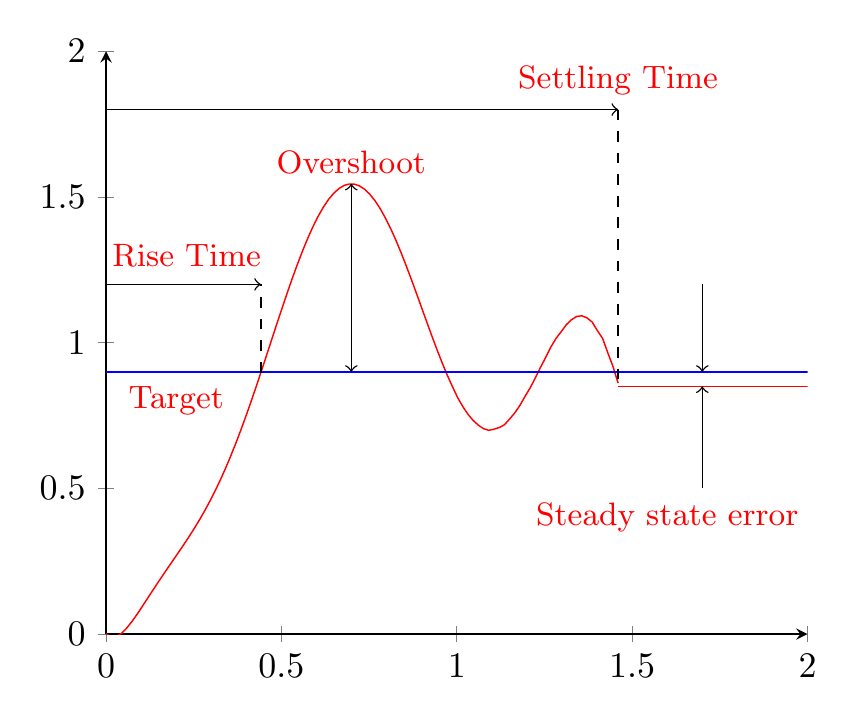
\begin{tikzpicture}[scale=1.3]
\begin{axis}[
    axis lines = left,
    xmin=0,xmax=2,
    ymin=0,ymax=2,
]

%Below the red parabola is defined
\addplot [
    domain=0:1.46, 
    samples=100, 
    color=red,
]
{80.83892322*x^8-473.66979127*x^7+1095.0629877*x^6-1265.55113227*x^5+768.48166718*x^4-242.51503181*x^3+39.47160828*x^2-1.30063244*x+0.00131008};

\addplot[color=red, domain=1.46:2] coordinates {
		(1.4598,0.85)
		(2,0.85)
};
\addplot[color=blue, domain=0:2] coordinates {
		(0,0.9)
		(2,0.9)
};
\addplot[<->,color=black, domain=0:2] coordinates {
		(0.69925398,1.5451)
		(0.69925398,0.9)
};

\node[red] at (axis cs:0.69925398,1.62){\small{Overshoot}};

\addplot[->,color=black, domain=0:2] coordinates {
        (1.7,1.2)
		(1.7,0.9)
};
\addplot[->,color=black, domain=0:2] coordinates {
        (1.7,0.5)
		(1.7,0.85)
};
\node[red] at (axis cs:1.6,0.4){\small{Steady state error}};

\addplot[color=black, domain=0:2, dashed] coordinates {
		(0.4415,0.8976)
		(0.4415,1.2)
};
\addplot[->,color=black, domain=0:2] coordinates {
		(0,1.2)
		(0.4415,1.2)
};
\node[red] at (axis cs:0.23,1.3){\small{Rise Time}};

\addplot[color=black, domain=0:2, dashed] coordinates {
		(1.4598,1.8)
		(1.4598,0.85)
};

\addplot[<-,color=black, domain=0:2] coordinates {
		(1.4598,1.8)
		(0,1.8)
};

\node[red] at (axis cs:0.2,0.8){\small{Target}};

\node[red] at (axis cs:1.4598,1.9){\small{Settling Time}};
\end{axis}
\end{tikzpicture}
\caption{PID properties.}\label{pidsettling}
\end{figure}

\subsection{PID Usage}
As the motors can only be controlled by setting a power percentage the PID controller was be used as an extra control layer. The PID controller is tuned by first using the Ziegler-Nichols method to create a stable system. Once a stable system has been found it will be fine tuned to avoid overshoot by using manual tuning. By lowering $K_p$ and $K_i$ the overshoot will decrease while the rise time increases. A compromise where to be found where the overshoot is small and the rise time is not too long.


\section{Sensors}\label{sec:dessensor}
The medium range infrared sensors are of the wide-angle type. At the tested distance of 45 centimeters they each have a field of view with a width of approximately 10 centimeters. The sensor readings are not entirely consistent throughout their field of view. There may be a large difference in the measured distance while the target is within this area. 
%To circumvent this issue the field of view of the sensor is split up into 4 zones as seen on \cref{sensorsections2} where each of the black bars represents an infrared sensor. These zones are based on the fact that the sensors consistently return bad distance readings at specific intervals. 

\begin{figure}[H]
\begin{center}
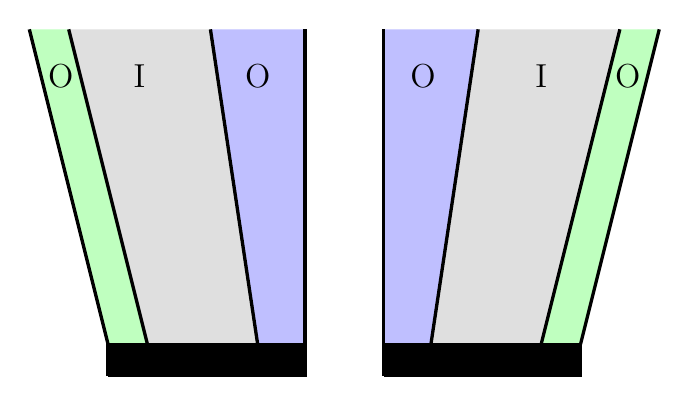
\begin{tikzpicture}

\fill[fill=green!25] (0,0.4) -- (-1,4.4) -- (-0.5,4.4) -- (0.5,0.4) -- (0,0.4); 
\fill[fill=gray!25] (0.5,0.4) -- (-0.5,4.4) -- (1.3,4.4) -- (1.9,0.4) -- (0.5,0.4);
\fill[fill=blue!25] (1.9,0.4) -- (1.3,4.4) -- (2.5,4.4) -- (2.5,0.4) -- (2,0.4);
\fill[fill=black] (0,0) -- (0,0.4) -- (2.5,0.4) -- (2.5,0) -- (0,0);

\fill[fill=green!25] (6,0.4) -- (7,4.4) -- (6.5,4.4) -- (5.5,0.4) -- (6,0.4);
\fill[fill=gray!25] (5.5,0.4) -- (6.5,4.4) -- (4.7,4.4) -- (4.1,0.4) -- (5.5,0.4);
\fill[fill=blue!25] (4.1,0.4) -- (4.7,4.4) -- (3.5,4.4) -- (3.5,0.4) -- (4.1,0.4);
\fill[fill=black] (3.5,0) -- (3.5,0.4) -- (6,0.4) -- (6,0) -- (3.5,0);

\draw[very thick] (0,0) -- (0,0.4) -- (2.5,0.4) -- (2.5,0) -- (0,0);
\draw[very thick] (3.5,0) -- (3.5,0.4) -- (6,0.4) -- (6,0) -- (3.5,0);

\draw[very thick] (2.5,0.4) -- (2.5,4.4);
\draw[very thick] (1.9,0.4) -- (1.3,4.4);
\draw[very thick] (0.5,0.4) -- (-0.5,4.4);
\draw[very thick] (0.0,0.4) -- (-1,4.4);

\draw[very thick] (3.5,0.4) -- (3.5,4.4);
\draw[very thick] (4.1,0.4) -- (4.7,4.4);
\draw[very thick] (5.5,0.4) -- (6.5,4.4);
\draw[very thick] (6,0.4) -- (7,4.4);

\node at (-0.6,3.8) {\large O};
\node at (0.4,3.8) {\large I};
\node at (1.9,3.8) {\large O};



\node at (4,3.8) {\large O};
\node at (5.5,3.8) {\large I};
\node at (6.6,3.8) {\large O};


%\draw[very thick] (2,4.8) -- (4,4.8);
%\draw[very thick] (2,4.6) -- (2,5);
%\draw[very thick] (4,4.6) -- (4,5);
%\node at (3,5.1) {\normalsize TRAIN};


\end{tikzpicture}
\caption{Infrared sensor detection zones.}
\label{sensorsections2}
\end{center}
\end{figure}

In \cref{sensorsections2} it is showed how the sensors field of view is split. A sensor is one of the black boxes with its field of view pointing upwards, the field of view is split up into 3 areas, the \textit{1} on both sides of a \textit{2} is seen as the same according to the sensors. However this can be used as an advantage that these fields exists. Through logic there can be made a difference between the \textit{1} on both sides of a \textit{2}. This will be used to split a sensors field of view into 3 different areas, this will help with tracking the target more precisely. It is then possible to see the train in three areas of a single sensor and to know when the train is between to sensors as shown on \Cref{sensorsections2} which will indicate that the train is in the middle.


%The \textit{1} and \textit{2} is how the sensors split, the \textit{0} shows that when it is inside both sensors field of view the train is in the middle. The \textit{-1} and \textit{1} farthest from the middle and closest to the middle is the same as far as the sensor goes. Using the sensors like this will result in a lot of faulty data. There for the decision was made to make the \textit{-1} and \textit{1} farthest from the middle count as a separate area which is 3. By doing this each of the sensors field of view is split into 3 different areas and it is easier to tell more precisely where the train is when moving past the sensors field of view. The \textit{0} is part of area \textit{1} next to it.     \\


%\Cref{sensorsections2} shows the sensors cone. It shows that a infrared sensor has 2 degrees it spots the target in. One of the problems is that on both sides of middle of the sensor it spots the target the same way. This is showed on graph \addtodo{Alex}{add graph to appendix and reference it graph of sensor readings for infrared} and is also depicted in \Cref{sensorsections2} by the 1 and -1 on both sides of 2 and -2. There are 2 sensors on the figure, the 1 and -1 furthest from the middle is handle like the 2 and -2 next to it. By using the sensors this way the train can be spotted in 5 different degrees, which are -2, -1, 0, 1, 2. This way the precision of where the train actually is compared to the sensors is increased. 

% Bad data consistently, used to split it into 'zones'
% Distance reading used to determine position
\section{Tracking}\label{sec:design_tracking}
%%%% Intro to tracking - Why is it needed? 
One of the primary tasks of the turret is tracking targets passing by in its observable area. Using the two-sensor setup, this tracking must preferably be done continuously in order to obtain as much information about the target as possible, by keeping the target within the sensors' field of view. This is done by having the rotation motor react to observations made by the sensors. \\

%%%% Naive approach
A very simple approach to this tracking problem, could be to simply activate the motor, turning it either left of right, based directly on each observation made by the sensors. The method could then be further refined by turning with different speeds, depending on the exact zone in which the target was observed. This approach might be effective if every observation provided by the sensors was perfectly accurate. \\

The sensors used for tracking are, however, not accurate, and produce noisy observations which may result in an incorrect estimate of the actual position of the target. If the turret were to act on these noisy observations, this might cause the turret to turn erroneously, possibly losing sight of the target, or overshooting and having to readjust immediately after. In order to improve the precision of the turret, the noisy observations have to be taken into account. For this purpose, different methods for reducing the impact of noisy observations are examined.

\subsection{Naive Bayes Classifier} \label{ss:naive_bayes}
%%%% Naive Bayes classifier
One possible approach for this could be to use a naive Bayes classifier. With this model, instead of directly reacting to an observation, the position of the target can be represented by a probability, distributed over several different possible positions~\cite{poole2010artificial}. The possible classes, contained in the class variable, would be all the possible speeds of the target. A binary feature variable would then exist for each of the possible positions within the observable area of the turret, where the binary value indicates whether the target was observed in the given position. This structure is shown in \cref{fig:bayes_classifier}. 

\begin{figure}[H]
\begin{center}
\begin{tikzpicture}

    \draw (3,3) circle [radius=0.5] node {$C$};
    
    \draw [-triangle 90,fill=black](2.75,2.55) --  (0.3,0.4);
    
    \draw (0,0) circle [radius=0.5] node {$F_1$};
    
    \draw [-triangle 90,fill=black](2.9,2.5) --  (2,0.5);

    \draw (2,0) circle [radius=0.5] node {$F_2$};

    
    \draw [-triangle 90,fill=black](3.35,2.6) --  (5.7,0.4);
    
    \draw (6,0) circle [radius=0.5] node {$F_k$};
    
    \draw [dotted, line width=1pt](2.6,0) --  (5.4,0);


\end{tikzpicture}
\end{center}
\caption{Graphical representation of a naive Bayes classifier.}
\label{fig:bayes_classifier}
\end{figure}

With this model it would be possible to predict the values of the class variable given evidence for some of the features using Bayes rule~\cite{poole2010artificial}. Each time a new observation is made, the probability in the classification variable would be updated. This model does, however, have limitations, such as quite large probability tables as well as a lack of native support of the temporal aspect that exists in the project~\cite{poole2010artificial}. Because of this, other models, with the temporal aspect included, will be considered instead.

%%%% Hidden markov model
\subsection{Hidden Markov Model} \label{ss:hmm}
A hidden Markov model (HMM) is a specialization of the more general dynamic Bayesian network, which is a Bayesian network where variables are related in respect to adjacent time steps \cite{poole2010artificial}. The model assumes the system to be a Markov process, where each state is dependent only on the previous state, meaning $P(x_k | x_0,x_1,...,x_{k-1}) = P(x_k | x_{k-1})$, where $x_k$ is the state of the system at discrete time step $k$~\cite{poole2010artificial}. This relation can be seen in \cref{fig:hmm}. 

\begin{figure}[H]
\begin{center}
\begin{tikzpicture}

    \draw [-triangle 90,fill=black](-1.5,2) --  (-0.5,2);
    
    \draw (0,0) circle [radius=0.5] node {$y_{k-1}$};
    \draw [-triangle 90,fill=black](0,1.5) --  (0,0.5);
    \draw (0,2) circle [radius=0.5] node {$x_{k- 1}$};
    
    \draw [-triangle 90,fill=black](0.5,2) --  (2.5,2);
    
    \draw (3,0) circle [radius=0.5] node {$y_{k}$};
    \draw [-triangle 90,fill=black](3,1.5) --  (3,0.5);
    \draw (3,2) circle [radius=0.5] node {$x_k$};
    
    \draw [-triangle 90,fill=black](3.5,2) --  (5.5,2);
    
    \draw (6,0) circle [radius=0.5] node {$y_{k+1}$};
    \draw [-triangle 90,fill=black](6,1.5) --  (6,0.5);
    \draw (6,2) circle [radius=0.5] node {$x_{k+1}$};
    
    \draw [-triangle 90,fill=black](6.5,2) --  (7.5,2);


\end{tikzpicture}
\end{center}
\caption{Graphical representation of the hidden Markov model for the system.}
\label{fig:hmm}
\end{figure}

By making this assumption, it is possible to predict the current state of the system, given only the prior state. Additionally, the model assumes that the state at each time step is not directly observable, instead an observation is associated with the state at each time step. By using the observation, the values of the hidden state variables can be estimated~\cite{poole2010artificial}. \\

Hidden Markov models are used in situations where certain information is necessary to obtain, without it being directly observable~\cite{ghahramani2001introduction}, as is the case in this project. While a HMM seems like a suitable solution, it does have certain limitations which would have to be accounted for. One such limitation is the assumption that the hidden state values in a HMM are discrete values~\cite{ghahramani2001introduction}. This is a disadvantage for this project, as the true state is continuous. This can be overcome by a discretization of the possible values for position and speed. As there are many possible positions and speeds, this will, however, result in a necessary construction of a large probability table. In an attempt to avoid this, an alternative without this limitation, namely the Kalman filter, is considered. 

%%%% Kalman filter
\subsection{Kalman Filter} \label{ss:kalman}
The Kalman filter is based on a hidden Markov model, with the difference that it is used for linear systems only, and the values in the hidden state are continuous rather than discrete \cite{faragher2012understanding}. While the Kalman filter does not require a Gaussian error distribution, in cases where the error is indeed Gaussian, the filter is an optimal estimator~\cite{kalman1960new}. The Kalman filter is very suitable for use in this project, as the assumption of a linear system holds, and the system can be modelled with high precision using this filter. Due to the filter working on continuous variables, the calculations can be done probabilistically using matrices, not requiring any probability tables, and due to the Markov assumption, only the matrices for the previous time step, and a current observation, are required for the computation, making it very suitable for an embedded real-time system~\cite{faragher2012understanding}. \\

%%%% The different processes/parts of the filter
Before the system, consisting of the turret and target, can be modelled, it is necessary to gain a better understanding of the functionality of the Kalman filter. Therefore, the vectors, matrices, and equations used in the calculations will first be examined. To distinguish vectors and matrices from scalars, vectors and matrices are denoted by bold font lower and upper case letters, respectively. The equations and theory used in the design of the Kalman filter is based on \cite{faragher2012understanding} and \cite{kalman1960new}. Before the equations used for calculating the estimated state are examined, the underlying assumption about the hidden true state is outlined.

\subsubsection{True State}
In a Kalman filter, it assumed that the evolution of the system's true state can be calculated according to the equation

\begin{equation}
\label{eq:state_equation}
  \vec{x}_k = \matr{F}_k \vec{x}_{k-1}+\matr{B}_k \vec{u}_k + \vec{w}_k \text{ ,}
\end{equation}

where $\vec{x}_k$ is the state vector, containing a set of continuous variables, representing the true state of the system at time $k$. These variables are assumed to be hidden in the Kalman filter. $\matr{F}_k$ is the state transition matrix, which describes how the state at time $k-1$ transitions into the state at time $k$. \\

$\vec{u}_k$ is the control vector, containing information about a known control input, such as acceleration, at time $k$. $\matr{B}_k$ is the control-input matrix, used to apply the effect of the control vector at time $k$ to the current state $\vec{x}_k$. \\

$\vec{w}_k$ is the process noise vector, containing continuous random variables representing the noise in the transition process for each state variable. As the random variables are continuous, their probability distribution is described by a probability density function (PDF). The noise is assumed to be white noise, with a Gaussian distribution. The variance of the noise vector at time $k$ is given by covariance matrix $\matr{Q}_k$, such that $\vec{w}_k \sim \mathcal{N}(0, \matr{Q}_k)$. \\

Measurements of the true state are made according to the equation

\begin{equation}
\label{eq:true_measurement}
  \vec{z}_k = \matr{H}_k \vec{x}_k + \vec{v}_k \text{ ,}
\end{equation}

where $\vec{z}_k$ is the measurement vector, containing the measurements of the true state at time $k$. $\matr{H}_k$ is the measurement transformation matrix, which maps the state vector into a measurement vector. This $\matr{H}_k$ matrix is necessary when the variables in the measurement vector do not directly correspond to the variables in the state vector. \\

$\vec{v}_k$ is the measurement noise vector, which contains continuous random variables, describing the noise in the measurement variables at time $k$. This noise is also assumed to be Gaussian distributed white noise, with variances given by covariance $\matr{R}_k$, such that $\vec{v}_k \sim \mathcal{N}(0, \matr{R}_k)$. \\

\subsubsection{Estimated State}
The Kalman filter generally estimates the state in a two-step process. First a prediction step, followed by an update step~\cite{faragher2012understanding}. The purpose of the predict step is to estimate the current true state, based on the previous prediction. In the update step a new observation is made, and the estimate is updated according to this observation. The update step takes into account the reliability of each measurement, and places more weight on measurements with a higher certainty~\cite{faragher2012understanding}. \\ 

In the prediction step, the state estimate at time $k$ is predicted, based on the previous estimate, by the equation

\begin{equation}
\label{eq:predict_state}
  \hat{\vec{x}}_{k|k-1} = \matr{F}_k \hat{\vec{x}}_{k-1|k-1} + \matr{B}_k \vec{u}_k \text{ ,}
\end{equation}

where $\hat{\vec{x}}_k$ is the state estimate vector, which represents the estimate of the true state at time $k$. This vector has the same dimensions as the true state, but here the variables are estimates, and thus subject to uncertainties. Therefore the variables in $\hat{\vec{x}}_k$ are continuous random variables, associated with a probability distribution represented by a PDF . The variance of the state estimate vector is given by covariance matrix $\matr{P}_k$. This covariance is predicted according to the equation 

\begin{equation}
\label{eq:predict_covariance}
  \matr{P}_{k|k-1} = \matr{F}_k \matr{P}_{k-1|k-1} \matr{F}_k^T + \matr{Q}_k \text{ .}
\end{equation}

Compared to \cref{eq:state_equation}, the process noise is omitted in \cref{eq:predict_state}. This omission is due to the noise being assumed to be white noise, and as such only the covariance in this noise $\matr{Q}_k$, included in \cref{eq:predict_covariance} is considered. The estimates predicted according to \cref{eq:predict_state,eq:predict_covariance} are called a priori estimates of the state and covariance, as they are not yet updated with the observation from time $k$. \\

In the update step the state and covariance predictions are updated with information from a new measurement. Both these updates rely on a Kalman gain matrix $\matr{K}_k$, that describes how much weight should be put on the prediction compared to the measurement. A high Kalman gain means the filter weighs the measurement higher, while a low Kalman gain means the filter weighs the estimate higher. This Kalman gain $\matr{K}_k$, is calculated using \cref{eq:kalman_gain}.

\begin{equation}
\label{eq:kalman_gain}
 \matr{K}_k = \matr{P}_{k|k-1} \matr{H}_k^T \big(\matr{H}_k \matr{P}_{k|k-1} \matr{H}_k^T + \matr{R}_k \big)^{-1}
\end{equation}

The state is updated with the new measurement according to \cref{eq:update_state}, and the covariance is updated according to \cref{eq:update_covariance}, where $\matr{I}$ is the identity matrix in the same dimensions as $\matr{P}_k$.

\begin{equation}
\label{eq:update_state}
  \hat{\vec{x}}_{k|k} = \hat{\vec{x}}_{k|k-1} + \matr{K}_k (\vec{z}_k - \matr{H}_k \hat{\vec{x}}_{k|k-1})
\end{equation}

\begin{equation}
\label{eq:update_covariance}
\begin{split}
    \matr{P}_{k|k} &= \matr{P}_{k|k-1} - \matr{K}_k \matr{H}_k \matr{P}_{k|k-1} \\
            &= (\matr{I} - \matr{K}_k \matr{H}_k) \matr{P}_{k|k-1}
\end{split}
\end{equation}

An overview of the two steps, along with the recursive nature of the Kalman filter, is shown in \cref{fig:kalman_filter}.

\imgscale{figures/kalman_filter.png}{Overview of the steps in the Kalman filter~\cite{kalman_figure}.}{fig:kalman_filter}{0.3}

The Kalman filter can be implemented using \cref{eq:kalman_gain,eq:update_state,eq:update_covariance}. In order to implement these equations, it is necessary to identify the $\matr{F}_k$, $\matr{B}_k$, $\matr{P}_k$, $\matr{Q}_k$ matrices, along with the $\vec{x}_k$, $\vec{u}_k$, and $\vec{z}_k$ vectors for a given system.

%%%% Modelling the system
\subsubsection{The System Model}
The hidden state of interest is the state of the target, particularly its position and speed. This results in the state estimate vector $\vec{x}_k$, shown in \cref{eq:state_vector}, with two continuous random variables. As the state estimate vector has two variables, it will have a 2-by-2 covariance matrix $\matr{P}_{k_{2,2}}$, shown in \cref{eq:covariance_matrix}, where $var(y_1)$ and $cov(y_1,y_2)$ denote the variance of a random variable, and the covariance between two random variables, respectively. 

\begin{equation}
\label{eq:state_vector}
  \vec{x}_k =
     \begin{bmatrix}
      x_k \\
      \dot{x}_k 
     \end{bmatrix}
    =
    \begin{bmatrix}
      position_k \\
      speed_k
     \end{bmatrix}
\end{equation}

\begin{equation}
\label{eq:covariance_matrix}
    \matr{P}_k =
    \begin{bmatrix}
      p_{k_{1,1}} & p_{k_{1,2}} \\
      p_{k_{2,1}} & p_{k_{2,2}}
    \end{bmatrix}
    =
    \begin{bmatrix}
      var(x_k) & cov(x_k, \dot{x}_k) \\
      cov(x_k, \dot{x}_k) & var(\dot{x}_k)
    \end{bmatrix}
\end{equation}

The speed of the target can not be measured by the sensors, so the measurement will consist of only a scalar $z_k$, which is the target's measured position, with a noise of $v_k$. This measurement is calculated by using the position of the turret at time $k$, denoted $c_k$, and adding the relative position measured by the sensors, see \cref{areas} in \cref{sec:dessensor}, here denoted $d_k$, giving 

\begin{equation}
\label{eq:relative_measurement}
  z_k = c_k+d_k
  \text{ .}
\end{equation}
 
The measured position maps directly into the state position, so disregarding the state's speed variable gives the measurement transformation matrix $\matr{H}_k$ shown in \cref{eq:measurement_transform}.

\begin{equation}
\label{eq:measurement_transform}
  \matr{H}_k =
     \begin{bmatrix}
      1 & 0 
     \end{bmatrix}
\end{equation}

Using this $\matr{H}_k$ matrix we obtain

\begin{equation}
\label{eq:measurement}
\begin{split}
  z_k &= \matr{H}_k \vec{x}_k + v_k \\
      &=
         \begin{bmatrix}
          1 & 0
         \end{bmatrix}
         \begin{bmatrix}
          x_{pos} \\
          \dot{x}_{vel} 
         \end{bmatrix}
         + v_k \\
     &= x_{pos} + v_k
     \text{ ,}
\end{split}
\end{equation}

which describes the connection between a measurement and a state. \\

As each target is assumed to be traveling at a constant speed, see \cref{sec:tracking}, the system has no known control input vector, so the control input matrix $\matr{B}_k$ and control vector $\vec{u}_k$ can be omitted, reducing \cref{eq:predict_state} to

\begin{equation}
\label{eq:reduced_predict_state}
  \hat{\vec{x}}_{k|k-1} = \matr{F}_k \hat{\vec{x}}_{k-1|k-1} \text{ .}
\end{equation}

Additionally, based on the assumption of a constant speed, it is assumed the system will not be subject to any significant noise between transitions. As such the process noise covariance $\matr{Q}_k$ will be zero, and thus \cref{eq:predict_covariance} can be reduced to

\begin{equation}
\label{eq:reduced_predict_covariance}
   \matr{P}_{k|k-1} = \matr{F}_k \matr{P}_{k-1|k-1} \matr{F}_k^T \text{ .}
\end{equation}

The state transition matrix $\matr{F}_k$ describes the change in the position and speed of the target between two consecutive time steps. The change in the target's position depends on the elapsed time since the previous state prediction, and the speed of the target, according to the equation $x_t = x_{t-1} + \dot{x}_{t-1} \Delta t $, while the speed remains constant, given by $\dot{x}_t = \dot{x}_{t-1}$. This can be rewritten in matrix form as

\begin{equation}
\label{eq:state_transition_calculation}
\begin{split}
  \begin{bmatrix}
  x_t \\
  \dot{x}_t
  \end{bmatrix}
      &=
  \begin{bmatrix}
    x_{t-1} + \dot{x}_{t-1} \Delta t \\
    \dot{x}_{t-1}
  \end{bmatrix}
  \\
      &=
     \begin{bmatrix}
      1 & \Delta t \\
      0 & 1
     \end{bmatrix}
     \begin{bmatrix}
      x_{t-1} \\
      \dot{x}_{t-1} 
     \end{bmatrix}
     \text{ ,}
\end{split}
\end{equation}

giving the state transition matrix

\begin{equation}
\label{eq:state_trans_matrix}
    \matr{F}_k =
    \begin{bmatrix}
      1 & \Delta t \\
      0 & 1
    \end{bmatrix}
    \text{ .}
\end{equation}

While the state estimate and state covariance are calculated at each iteration of the filter, initial values must be specified. The initial position will be equal to the first possible measurement of the target, with some small amount of variance, and can therefore be calculated according to \cref{eq:relative_measurement}. The turret always starts in position zero, giving the initial turret position $c_0=0$. The target will always be moving from right to left, and so the first observation will always be made in zone $2$, giving the initial relative measurement $d_0=-20.74$. The initial position $x_0$ can then be approximated by $x_0 = c_0+d_0$. As this approximation will be relatively accurate, its initial variance will be low. As long as the variance is relative low, the exact value does not have a large impact. As such the initial variance $var(x_0)$ is specified as $p_{0_{1,1}} = 1$. \\

The speed of the target is controlled discretely, and can in general have $i$ possible discrete values $s_1, s_2, \dots, s_i$. In practice, observations have shown the speed to be continuous. This variation will, however, be disregarded when specifying the initial speed. Assuming an equal probability of the target's possible speeds, the most accurate initial speed can be specified as the mean of these speeds, given by $\bar{s}=(s_1+s_2+\dots+s_i)/i$.  \\

If the initial speed is specified as the expected value $\bar{s}$, and this initial value is to have an impact on the speed prediction, the variance would have to be relatively low. This is, however, problematic as the actual speed is not known, and will as such be subject to uncertainties. Alternatively, the initial speed might simply be specified as an arbitrary, somewhat realistic, value, with a high variance accounting for the inaccurate value. The Kalman filter is very effective at dealing with uncertainties, consequently favoring the latter alternative method. As such the initial speed will simply be set as an arbitrary value of 50 degrees per second matching the measured speed at the second speed setting. This gives the initial state

\begin{equation}
\label{eq:initial_state}
\begin{split}
    \mathbf{x_0} &=
    \begin{bmatrix}
      x_0 \\
      \dot{x}_0 
    \end{bmatrix}
    \\
    &=
    \begin{bmatrix}
      c_0+d_0 \\
      50
    \end{bmatrix}
    \\
    &=
    \begin{bmatrix}
      -20.74 \\
      50
    \end{bmatrix}
    \text{ .}
\end{split}
\end{equation}

As the actual speed is unknown, and the initial speed was chosen arbitrarily, the variance of the initial speed will be high. Again, the exact value is not very important, but as the largest difference between the initial and the two other possible speeds is $30$ degrees per second, the initial variance is specified as this value squared, giving $p_{0_{2, 2}} = 30^2$. As the the state variables are independent of each other, the covariance is set as $p_{0_{1,2}}=p_{0_{2,1}}=0$. This gives the initial covariance matrix

\begin{equation}
\label{eq:initial_covariance}
\begin{split}
    P_0 &=
    \begin{bmatrix}
      p_{1,1} & p_{1,2} \\
      p_{2,1} & p_{2,2}
    \end{bmatrix}
    \\
    &=
    \begin{bmatrix}
      1 & 0 \\
      0 & 30^2
    \end{bmatrix}
    \\
    &=
    \begin{bmatrix}
      1 & 0 \\
      0 & 900
    \end{bmatrix}
    \text{ .}
\end{split}
\end{equation}

Based on this model, a Kalman filter can be implemented for the system. In particular the filter can be implemented using the $\matr{H}_k$, $\matr{F}_k$, and $\matr{P}_0$ matrices specified in \cref{eq:measurement_transform,eq:state_trans_matrix,eq:initial_covariance}, along with the $\vec{x}_0$ vector from \cref{eq:initial_state}, with a predict step using \cref{eq:reduced_predict_state,eq:reduced_predict_covariance}, and an update step using \cref{eq:kalman_gain,eq:update_state,eq:update_covariance}.
\section{Shooting}
The shooting system handles the matter of aiming, which boils down to finding and adjusting to a trajectory prediction, as well as the time sensitive aspect of shooting while the aim is on target. In the design of the turret, see \cref{turret}, the physical shooting mechanism is described, which provides the frame, within which the shooting system can operate. In this section the design solutions for these problems will be explained.

\subsection{Trajectory Prediction}
When aiming, the PID controller will handle turning to the estimated position, and as such the process is reduced to finding that position, also known as the trajectory prediction.

Then there is the matter of accuracy of the fired projectiles, which was considered to be good enough to not warrant consideration when aiming. This was tested by placing the turret 75 centimeters away from a circular target with a diameter of 5 centimeters. At this distance a projectile drop off of 10 centimeters was recorded. A total of 10 projectiles were fired and all of them managed to hit the target. The hits were not centered in one location, but spread about the target within the 5 centimeter boundary.

In the preliminary design \cref{predesign:shoot}, the concern of compensating for the travel time and launch of the projectile, is considered to be a matter of calculating the correct offset. The correct offset will be changing along with the speed of the target, and as such the offset should be a function of the speed. However, this alone would cause the turret to offset violently during the process of finding the correct speed, as the estimated speed often varies greatly in the early iterations of the Kalman filter. This can contribute unnecessary noise to the readings, as the sensor zones closest to the center of the turret, are the most precise. \\

This could be solved by applying the offset after a certain stability has occurred. However this could turn out to be too slow of a reaction, since this would cause the turret to suddenly accelerate to compensate, which in turn could result in overshooting by the PID controller and thus of the projectile. Instead the offset should be applied gradually, as the turret hones in on the target. \\

This is suggested to be done by having the offset function not only be a function of the speed but also of the determinant of the $\matr{P}_k$ matrix, found in the Kalman filter. Since this determinant approaches 0 along with the Kalman filter's \enquote{certainty} of its estimate, a function similar to this could be used:

\begin{equation}
  f(speed,det(\matr{P}_k)) = \frac{speed*n}{1+e^{-k*(\frac{1}{det(\matr{P}_k)}-x0)}}
\label{eq:logic}
\end{equation}

The function in \cref{eq:logic} is a logistic function. An example of a logistic function is shown plotted in \cref{fig:logic}. As shown on the figure the function is upper bounded, which in \cref{eq:logic} is $speed*n$. This causes the offset to be bounded based on the speed of the target. $k$ is a constant determining the steepness of the function. $x0$ is the sigmoid's midpoint which is shown as the black line in \cref{fig:logic}. This point influences when the curve should start growing with a higher steepness. In this project $x0$ is used to control when the offset should be high enough to influence the turret's position. $(1/(det(\matr{P}_k))$ is not linear, but exponential which causes the function to have a higher steepness. This increase in the steepness can be compensated for by lowering $k$. 


\begin{figure}[H]
\centering
\begin{tikzpicture}
    \begin{axis}
    \addplot[mark=none, very thick] coordinates{(9,5.5) (9,4.5)};
    [
        grid=major,     
        xmin=0,
        xmax=15,
        axis x line=bottom,
        ytick={5,10},
        ymax=10,
        axis y line=middle,
    ]
        \addplot%
        [
            blue,%
            mark=none,
            samples=100,
            domain=-0:15,
        ]
        (x,{10/(1+2.718^(-1*(x-9)))});
    \end{axis}
\end{tikzpicture}
\caption{Plot of a logistic function}
\label{fig:logic}
\end{figure}

\subsection{Timing a Shot}
When the system has settled on an estimate of the target's position, it will not necessarily keep the aim on point for long. This can either be due to the expected errors in the PID controller or simply since the target will eventually exit the observable area. Therefore, the launch of a shot requires timing. 

\subsubsection{Cocking}
In order to minimize the delay between reaching the desired aim and launching a projectile, the turret has a cocking function. The cocking function, which borrows its name from the act of cocking a hammer on a revolver, retracts the piston partially from the chamber, such that less motion, and therefore time, is required to reach the apex of the retraction. Optimally, cocking would bring the piston on the edge of the apex, such that it would only require a minimal amount of motion to release a shot. However, since the motors cannot be locked in position, the PID controller would be trying to stabilize them against the increasing pull of the elastic bands. This would make the cocking rather unstable and unpredictable with the current PID controller. Therefore, it was instead decided to cock at the position where the elastic bands start to exert a pull in order to achieve consistency and stability at the cost of some speed. \\

Alternatively, a mechanical one way clutch combined with a non-reversing PID controller could have been used to stabilize the system at the apex \cite{clutch}.

\subsubsection{Fire} 
Firing a projectile is a rather simple process and is done by rotating the firing rods past the apex. However, since the PID controller tries to stop at the position it is given, and thus slows down when nearing its target, the fire function must provide a target well past the apex. The retained use of the PID controller is to allow for continuous fire, which is done by having the fire function rotate to the next point of cocking.

% this is just the preliminary design tekst \label{predesign:shoot}
%The last part of the preliminary design will consider trajectory prediction. The actual processes of aiming and shooting will not be covered in the preliminary since they are trivial when hardware factors are not involved, and are even then primarily implementation problems. Trajectory prediction does however deserve a mentioning. Given that the target is being tracked correctly, and thus our predictions on positions and velocity are correct, the right trajectory can be calculated given information on projectile speed and launch delays. But remembering that this process involves mechanical movement which is prone to inaccuracies (at least from a mathematical standpoint) a margin of error is expected. This includes the angle of the target relative to the turret, the width of the target, and whether the tracked point of the target is closer to the front of the target or the rear.\\








%måske skal kalman gain bruges til offset i stedet for diskriminanten?






















%\section{Summary}
In the PID $\Delta t$ is integrate into the coefficients there the PID will only work on that specific speed, therefor when implementing it the speed at which it is set. The sensors need to pull at a of 6 milliseconds to make sure that the target don't jump from one to a zone that is not abjected without the sensors getting a measurement. Floating point would be nice to have for many of the calculations, as some of them might get so small that integer persion wont suffice, this could be handle my multiplying with a larger value and use that for the calculation, but float will make the code more readable. Both the PID, the Kalman filter and shooting is time sensitive, therefor a normal OS cant be used as there are no guarantee that a given task will run exactly when it is called.\addtodo{Lasse}{Det her skal skrives helt om...}


